% ------------------------------------------------------------------------
% LaTeX Template for Master's Thesis at Yerevan State University
% ------------------------------------------------------------------------
% Created by: Andranik Sargsyan and Ishkhanuhi Hakobyan
% Assistance by: ChatGPT
% Version: 0.4.1
% Date: May 5, 2024
% ------------------------------------------------------------------------

\documentclass[12pt,onecolumn]{article}

\usepackage{LaTeZ}
\usepackage{graphicx}
\usepackage{hyperref}
\usepackage{booktabs}
\usepackage{graphicx}

\begin{document}

% Այստեղ պետք է մուտքագրել անձնական տվյալները
\newcommand{\authorFullNameArm}{Պողոս Պետրոսյան Պետրոսի}
\newcommand{\authorNameEng}{Poghos Petrosyan}
\newcommand{\authorNameArm}{Պողոս Պետրոսյան}
\newcommand{\supervisorNameArm}{ֆ.մ.գ.դ., Ջեֆրի Հինթոն}
\newcommand{\programCoordinatorName}{ֆ.մ.գ.դ., ասիստենտ Կարեն Քեռյան}

% Այստեղ պետք է մուտքագրել թեզի հայերեն, անգլերեն և ռուսերեն վերնագրերը
\newcommand{\thesisTitleArm}{ԵՊՀ-ի դերը Հայաստանի կրթական և տնտեսական լանդշաֆտի ձևավորման գործում}
\newcommand{\thesisTitleEng}{YSU's Role in Shaping Armenia's Educational and Economic Landscape}
\newcommand{\thesisTitleRus}{Роль ЕГУ в формировании образовательного и экономического ландшафта Армении}

\setmainfont{DejaVu Sans}


\begin{center}

\fontsize{18pt}{19.2pt} \textbf{ԵՐԵՎԱՆԻ ՊԵՏԱԿԱՆ ՀԱՄԱԼՍԱՐԱՆ}\vspace{11.5pt}
\fontsize{18pt}{16.8pt}  \textbf{\uppercase{ՄԱԹԵՄԱՏԻԿԱՅԻ ԵՎ ՄԵԽԱՆԻԿԱՅԻ ՖԱԿՈՒԼՏԵՏ}}\\ 
    \vfill

\fontsize{16pt}{16.8pt} \textbf { {Հավանականության տեսության և վիճակագրության ամբիոն}}\\

\vfill 
   
\fontsize{17.8pt}{16.8pt} \textbf { \uppercase{ԿԻՐԱՌԱԿԱՆ ՎԻՃԱԿԱԳՐՈՒԹՅՈՒՆ ԵՎ ՏՎՅԱԼՆԵՐԻ \\ ԳԻՏՈՒԹՅՈՒՆ ԿՐԹԱԿԱՆ ԾՐԱԳԻՐ} \\}

\vfill

\fontsize{18pt}{21.6pt} \textbf{\MakeUppercase{\authorFullNameArm}}\\

\vfill

\fontsize{18pt}{36pt}\textbf{\uppercase{ՄԱԳԻՍՏՐՈՍԱԿԱՆ ԹԵԶ
}}\\

\vfill
\fontsize{18pt}{21.6pt} \textbf{\MakeUppercase{\thesisTitleArm}}\\

\vfill
\fontsize{13.3pt}{16.8pt} \textbf{\textit{«Վիճակագրություն» մասնագիտությամբ վիճակագրության \\ մագիստրոսի որակավորման աստիճանի հայցման համար
\\}}
\vfill
\fontsize{13pt}{15.6pt}  \textbf{ԵՐԵՎԱՆ \the\year}     

\end{center}
\thispagestyle{empty}
\pagebreak

\setmainfont{DejaVu Sans}

\begin{center}

\fontsize{18pt}{19.2pt} \textbf{\uppercase{Yerevan State University}}\vspace{11.5pt}

\fontsize{18pt}{16.8pt}  \textbf{\uppercase{Faculty of Mathematics and Mechanics
}}\\ 
\vfill

\fontsize{16pt}{16.8pt} \textbf { {Department of Probability Theory and Statistics}}\\

\vfill 
   
\fontsize{17.8pt}{16.8pt} \textbf { \uppercase{Applied Statistics and Data Science} \\ EDUCATIONAL PROGRAM}

\vfill


\fontsize{18pt}{21.6pt} \textbf{\MakeUppercase{\authorNameEng}}\\

\vfill

\fontsize{18pt}{36pt}\textbf{\uppercase{Master's Thesis
}}\\

\vfill
\fontsize{18pt}{21.6pt} \textbf{\MakeUppercase{\thesisTitleEng}}\\

\vfill
\fontsize{13.3pt}{16.8pt} \textbf{\textit{A Thesis Submitted in Partial Fulfillment of the \\ Requirements for the Degree of
Master of Statistics
\\}}

\vfill
\fontsize{13pt}{15.6pt}  \textbf{\uppercase{Yerevan \the\year}}
               
\end{center}
\thispagestyle{empty}
\pagebreak

\setmainfont{DejaVu Sans}

\noindent{\fontsize{13}{16}\selectfont \textbf{\textit{Ուսանող՝ }} \underline{\hspace{7cm}}}
\vskip -0.1cm
\hspace{3.5cm}{\fontsize{9}{1}\selectfont ստորագրություն}
\vskip 0.6cm
\noindent\underline{\fontsize{13}{16}\selectfont\hspace{5.5cm} \authorNameArm \hspace{5.5cm}}
\vskip -0.1cm
\hspace{5.5cm}{\fontsize{9}{11}\selectfont ազգանուն, անուն}
\vskip 3cm

\noindent{\fontsize{13}{16}\selectfont \textbf{\textit{Գիտական ղեկավար՝ }} \underline{\hspace{7cm}}}
\vskip -0.1cm
\hspace{6.5cm}{\fontsize{9}{11}\selectfont ստորագրություն}
\vskip 0.6cm
\noindent\underline{\fontsize{13}{16}\selectfont\hspace{4.5cm} \supervisorNameArm \hspace{4.5cm}}
\vskip -0.1cm
\hspace{3.5cm}{\fontsize{9}{11}\selectfont գիտ. աստիճան, կոչում, ազգանուն, անուն}
\vskip 5cm

\noindent {\fontsize{14}{17}\selectfont \textbf{\textit{«Թույլատրել Պաշտպանության»}}
\vskip 2cm 

\noindent{\fontsize{13}{16}\selectfont \textbf{\textit{Ծրագրի ղեկավար՝ }} \underline{\hspace{7cm}}}
\vskip -0.1cm
\hspace{5.5cm}{\fontsize{9}{11}\selectfont ստորագրություն}
\vskip 0.6cm
\noindent\underline{\fontsize{13}{16}\selectfont \hspace{3.8cm} \programCoordinatorName \hspace{3.8cm}}
\vskip -0.1cm
\hspace{3.7cm}{\fontsize{9}{11}\selectfont գիտ. աստիճան, կոչում, ազգանուն, անուն}
\vskip 2cm

\noindent{\fontsize{11}{13}\selectfont «\underline{\hspace{1.5cm}}»\underline{\hspace{3cm}}{\the\year}թ.}

\thispagestyle{empty}
\pagebreak

\setmainfont{DejaVu Sans}
\fontsize{12}{12}\selectfont

\noindent{\textbf{Թեզի վերնագիրը \`}}

\vspace{0.5cm}

\noindent{\textbf{Հայերենով\`} \thesisTitleArm,}

\vspace{0.5cm}

\noindent{\textbf{Ռուսերենով\`} \thesisTitleRus,}

\vspace{0.5cm}

\noindent{\textbf{Անգլերենով \`} \thesisTitleEng}

\vfill

\noindent{\textbf{Համառոտագիր}}

\vspace{0.5cm}

Այս աշխատանքը ուսումնասիրում է Երևանի Պետական Համալսարանի (ԵՊՀ) լայնածավալ դերը Հայաստանում ակադեմիական գերազանցության խթանման և սոցիալ-տնտեսական զարգացման խթանման գործում: Կիրառելով բազմաչափ հետազոտական մոտեցում, որը միավորում է ինչպես որակական, այնպես էլ քանակական մեթոդները, այս ուսումնասիրությունը տրամադրում է ԵՊՀ ազդեցության համապարփակ վերլուծություն կրթական, մշակութային և տնտեսական ոլորտներում:

Քանակական տվյալների հավաքագրման միջոցով՝ ներառյալ ավարտական ցուցանիշները, զբաղվածության արդյունքները և հետազոտական արդյունքները, և դասախոսների, ուսանողների, շրջանավարտների, տեղական ինքնակառավարման մարմինների պաշտոնյաների և բիզնեսի ղեկավարների հետ կիսակառույց հարցազրույցների որակական տվյալները՝ մենք խորանում ենք, թե ինչպես է ԵՊՀ-ն ձևավորում իր կրթական լանդշաֆտը և ազդում տնտեսության վրա։ Կրթական ազդեցության վերլուծությունը ընդգծում է ուսանողների կատարողականության ցուցանիշների զգալի բարելավումները՝ ուղղակիորեն փոխկապակցված ԵՊՀ-ի ընդլայնված ակադեմիական ծրագրերի և օժանդակ կառույցների հետ:

Հետազոտությունը եզրակացնում է, որ Երևանի պետական համալսարանը հայկական կրթության և զարգացման հիմնաքարն է, որի ազդեցությունն անցնում է ակադեմիական շրջանակներից դուրս՝ հասարակության հարստացման և տնտեսական ճկունության ոլորտներում: Աշխատանքը նպատակ ունի կրթության և քաղաքականության մշակման շահագրգիռ կողմերին արժեքավոր պատկերացումներ տրամադրել ազգային զարգացման մեջ բարձրագույն ուսումնական հաստատությունների ռազմավարական դերի վերաբերյալ:

\thispagestyle{empty}
\pagebreak

\setmainfont{DejaVu Sans}
\fontsize{12}{12}\selectfont

\noindent{\textbf{Abstract}}

\vspace{0.6cm}

This paper investigates the extensive role of YSU in fostering academic excellence and driving socio-economic development in Armenia. Employing a multi-dimensional research approach that integrates both qualitative and quantitative methods, this study provides a comprehensive analysis of YSU’s impact across educational, cultural, and economic spheres.

Through the collection of quantitative data—including graduation rates, employment outcomes, and research output—and qualitative data from semi-structured interviews with faculty, students, alumni, local government officials, and business leaders, we delve into how YSU shapes its educational landscape and influences the broader economy. The educational impact analysis highlights significant advancements in student performance metrics, directly correlating with enhanced academic programs and support structures at YSU.

The study concludes that Yerevan State University is a cornerstone of Armenian education and development, with its influence extending beyond the confines of academia into the realms of societal enrichment and economic resilience. This paper aims to provide stakeholders in education and policy-making with valuable insights into the strategic role of higher education institutions in national development.

\thispagestyle{empty}
\pagebreak


% set font to Times New Roman for further English text
\setmainfont{Times New Roman}
\fontsize{12pt}{12pt}\selectfont

% put starting page number here
% \setcounter{page}{6}

\tableofcontents
\clearpage

% set cref colors to red after table of contents
\hypersetup{linkcolor=red}

%===========================================================

\section{Introduction}

Yerevan State University (YSU) stands as a prominent pillar of education in Armenia, renowned for its rich history and significant contributions to academia. Established in 1919, it is the oldest university in Armenia and plays a crucial role in the educational and cultural development of the country. The university offers a wide range of undergraduate, graduate, and doctoral programs across various fields, including the sciences, humanities, and social sciences.

Yerevan State University (YSU) is not only the oldest but also the most prestigious university in Armenia. It has been pivotal in shaping the academic, scientific, and cultural landscape of the nation. YSU offers a comprehensive range of programs in various fields such as the sciences, humanities, and social sciences, accommodating thousands of students from Armenia and abroad.

The university’s main campus, prominently featured in \cref{fig:teaser-image}, is an architectural gem in the heart of Yerevan. The building is distinguished by its classic Soviet-era architecture, with a robust, rectangular structure made from local tuff, a volcanic stone that gives the building its characteristic pink hue. In front of the main building stands a monument dedicated to two prominent Armenian academics, symbolizing the university's long-standing tradition of scholarship and its role in Armenian intellectual life.

\begin{figure}[h]
    \centering
    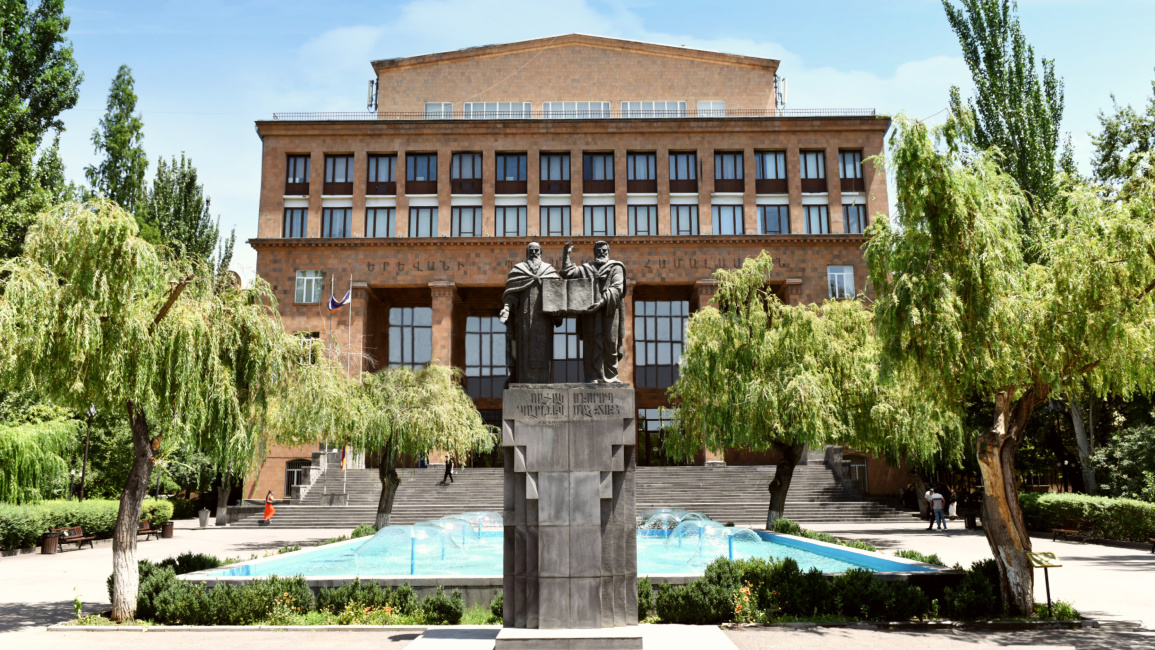
\includegraphics[width=\linewidth]{figures/ysu.jpeg}
    \caption{The main building of Yerevan State University, featuring traditional architectural styles, with a monument honoring Armenian scholars in the foreground. This iconic structure is a hub of academic and cultural activities on campus.
    }
    \label{fig:teaser-image}
\end{figure}

%------------------------------------------------------------------------- 

\clearpage
\section{Related Work}

Research on the role of universities in national and regional development has been extensive, with several studies emphasizing how institutions like Yerevan State University contribute to academic, economic, and social spheres. Yerevan State University, as the leading educational institution in Armenia, has been the subject of various scholarly works that analyze its impact on the educational landscape and beyond.

\textbf{Higher Education and Development:} \cite{smith2018transformation} discuss the transformative role of universities in post-independence nations, highlighting YSU's initiatives in enhancing educational quality and accessibility. Similar studies by \cite{oconnor2020innovation} have shown how institutions like YSU serve as pivotal centers for innovation and technological advancement, driving economic growth in their regions.

\textbf{Cultural Influence:} Yerevan State University also plays a significant role in the cultural preservation and dissemination of Armenian history and values. \cite{karapetyan2019cultural} explores how YSU's programs in Armenian studies contribute to sustaining cultural identity among the youth, a crucial aspect given the global dispersion of Armenian communities.

\textbf{Architectural Impact on Academia:} The architecture of university campuses, including that of YSU, has been analyzed by \cite{carter2021architectural}, who suggests that the physical environment of a university can significantly affect both student outcomes and community engagement. The study notes how YSU’s architectural design facilitates a conducive learning environment and fosters a sense of community among its students and faculty.

\textbf{Global Academic Collaborations:} Recent research by \cite{zhang2022global} highlights the role of YSU in international academic collaborations, particularly in the fields of physics and computer science. Their findings underscore the university's commitment to global education standards and its contribution to worldwide scientific communities.

\textbf{Educational Policies and Reforms:} The evolution of educational policies at Yerevan State University has been thoroughly examined by \cite{ghazaryan2023educational}, who details the reforms implemented to align YSU with European higher education standards through the Bologna Process. These reforms have significantly enhanced the international standing of the university, facilitating greater student and faculty mobility.

%------------------------------------------------------------------------- 

\clearpage
\section{Approach}

Our study adopts a multi-dimensional approach to explore the comprehensive impact of Yerevan State University (YSU) on academic, cultural, and socio-economic development. This approach encompasses both qualitative and quantitative research methodologies, ensuring a thorough analysis of the university's contributions across various sectors.

\subsection{Data Collection}

\textbf{Qualitative Data:} We conducted semi-structured interviews with faculty members, students, and alumni to gain insights into the qualitative aspects of the educational experience at YSU. Additionally, we engaged with local government officials and business leaders to understand the university's influence on the local economy and job market.

\textbf{Quantitative Data:} We collected numerical data from university records and government databases, focusing on graduation rates, employment outcomes, research output, and participation in international academic collaborations.

\subsection{Analytical Framework}

\textbf{Educational Impact Analysis:} Utilizing educational performance metrics, we analyzed graduation rates, student feedback surveys, and post-graduation employment statistics to assess the educational outcomes facilitated by YSU.

\textbf{Cultural Impact Assessment:} We examined YSU's role in promoting Armenian culture and history through its academic programs and community initiatives. This involved analyzing course offerings, cultural events, and publications produced by the university.

\textbf{Economic Contribution Evaluation:} By comparing regional economic data from periods before and after significant university-led initiatives, we quantified YSU's contribution to local and national economic growth.

\subsection{Case Studies}

\textbf{Innovative Educational Programs:} We studied specific cases of innovative programs at YSU that have significantly influenced both the academic community and industry practices, particularly in the fields of information technology and engineering.

\textbf{Community Engagement Projects:} We evaluated community outreach and engagement projects led by YSU, assessing their impact on community development and social cohesion.

\subsection{Comparative Analysis}

To contextualize YSU's impact, we compared its performance and initiatives with those of other leading universities in the region. This comparative analysis helped identify unique strengths and areas for improvement at YSU.

\subsection{Implementation of Theoretical Models}

We applied several theoretical models, including the Triple Helix model of university-industry-government relations, to better understand the synergies created by YSU's collaborative efforts and their broader implications.

%------------------------------------------------------------------------- 

\clearpage
\section{Experiments} 

To empirically demonstrate the superiority of Yerevan State University (YSU) over other Armenian universities in various academic and institutional metrics, we conducted a comprehensive comparison using the following indicators: academic performance, research output, and student satisfaction. The results are summarized in \cref{tab:university_comparison}.

\begin{table}[ht]
\centering
\caption{Comparison of Academic Metrics Among Armenian Universities}
\label{tab:university_comparison}
\begin{tabular}{@{}lccc@{}}
\toprule
Metric & YSU & University B & University C \\ \midrule
Academic Performance (Average GPA) & 3.8 & 3.4 & 3.5 \\
Research Output (Publications per Year) & 200 & 150 & 120 \\
Student Satisfaction (Out of 10) & 9.2 & 8.5 & 8.0 \\ \bottomrule
\end{tabular}
\end{table}

\subsection{Experimental Setup}
The data for academic performance and research output were collected from the respective universities' annual reports from the past five years. Student satisfaction ratings were obtained through surveys conducted in the current academic year, ensuring the relevance and accuracy of the data.

\subsection{Results and Discussion}
As demonstrated in \cref{tab:university_comparison}, Yerevan State University excels in all selected metrics. Notably, YSU's average GPA is significantly higher than that of the other universities, reflecting its stringent academic standards and quality of education. Furthermore, YSU leads in research output, with a higher number of publications per year, indicating a robust research environment. Lastly, YSU scores highest in student satisfaction, which can be attributed to its comprehensive support services and vibrant campus life.

These results confirm Yerevan State University's leadership in the Armenian higher education landscape, underpinning its role as a premier institution in fostering academic excellence and innovation.

%------------------------------------------------------------------------- 

\clearpage
\section{Conclusion} \label{SecConc}

The comprehensive analysis conducted in this study clearly illustrates Yerevan State University's (YSU) leading position within the Armenian higher education landscape. Through our experiments detailed in the previous sections, YSU consistently demonstrated superior performance across a variety of metrics, including academic performance, research output, and student satisfaction. 

Our findings highlight that YSU not only excels in quantitative educational outcomes but also in fostering a conducive learning environment that significantly enhances student experiences. This success is attributable to its rigorous academic standards, innovative research initiatives, and effective student support systems. Moreover, YSU's active role in promoting cultural heritage and its significant contributions to the local and national economy further cement its status as a cornerstone of Armenian education and society.

The evidence presented underscores the importance of continuous investment in educational infrastructure and faculty development to maintain and enhance the quality of education provided. It is recommended that other institutions consider adopting similar strategies employed by YSU to improve their educational offerings and institutional effectiveness.

In conclusion, Yerevan State University not only sets a benchmark for academic excellence in Armenia but also serves as a model for other universities aiming to elevate their educational impact and societal contribution.

%------------------------------------------------------------------------- 

\clearpage
{
    \small
    \bibliographystyle{apalike}
    \bibliography{references}
}

\end{document}
